\documentclass[12pt]{article}
\usepackage{geometry}
\geometry{a4paper, left=25mm, right=25mm}
\usepackage{graphicx}
\usepackage{amsmath}
\usepackage[slovene]{babel}
\usepackage{placeins}
\graphicspath{ {./Imgs/} }
\begin{document}

\title{\textbf{Izračun porazdelitve temperature v 2D prerezih} \\
\large Projektna naloga pri predmetu Napredna računalniška
orodja}
\author{Kristijan Danov 23221364, Rade Blagojević 23221382}
\date{Januar, 2025}
\maketitle
\thispagestyle{empty}

\newpage

\newpage

\renewcommand*\contentsname{Kazalo vsebine}
\tableofcontents
\renewcommand{\listfigurename}{Kazalo slik}
\listoffigures

\newpage

\section{Uvod}

\subsection{Prenos toplote v 2D prerezu}
V tem projektu smo obravnavali časovno ustaljen problem prenosa toplote v 2D prerezu, kjer smo za dane robne pogoje izračunali temperaturni gradient prereza. V tem primeru smo predpostavili neodvisno toplotno prevodnost in robne pogoje ter smo zanemarili notranjo generacijo toplote. Tak primer prenosa toplote po trdini je definiran kot
$$\frac{\partial}{\partial x}(k \frac{\partial T}{\partial x})+\frac{\partial}{\partial y}(k \frac{\partial T}{\partial y})+q=0$$

\subsection{MKR Metoda reševanja}
Za reševanje kopleksnih primerov diferencialnih enačb pogosto posežem k numeričnim metodam saj analitično reševanje ni mogoče. Nekatere od najbolj znanih metod numeričnega reševanja so:
\begin{itemize}
    \item metoda končnih razlik (MKR)
    \item metoda končnih elementov (MKE)
    \item metoda končnih volumnov (MKV)
    \item metoda robnih elementov (MRE)
\end{itemize}
Projekt smo naredili spomočno metode končnih razlik. Diferencialno enačbo iskane
funkcije v danem prostoru rešujemo numerično tako, da odvode funkcije aproksimiramo s diferenčne sheme.
\newline
Pri tej metodi moramo
obravnavano območje popisati s strukturirano mrežo pravokotnikov. V robnih točkah pa definiramo vnaprej predpisane pogoje.

\subsubsection{Robni pogoji pri aproksimaciji temperature spomočjo metode MKR}
Prestop toplote na notranjem kotu
$$2(T_{m-1,n}+T_{m,n+1})+(T_{m+1,n}+T_{m+1,n-1})+2\frac{h \Delta x}{k}T_{ext}-2(3+\frac{h\Delta x}{k})T_{m,n}=0$$
Prestop toplote na robu
$$2(T_{m-1,n}+T_{m,n+1}+T_{m,n-1})+2\frac{h\Delta x}{k}T_{ext}-2(\frac{h\Delta x}{k}+2)T_{m,n}=0$$
Prestop toplote na zunanjem kotu
$$2(T_{m-1,n}+T_{m,n-1})+2\frac{h\Delta x}{k}T_{ext}-2(\frac{h\Delta x}{k}+1)T_{m,n}=0$$
Toplotni tok na robu
$$(2T_{m-1,n}+T_{m,n-1}+T_{m,n+1})+2\frac{q\Delta x}{k}-4T_{m,n}=0$$
Vozlišče v notranjosti
$$T_{m-1,n}+T_{m+1,n}+T_{m,n-1}+T_{m,n+1}-4T_{m,n}=0$$

\subsubsection{Rešitev sistema enačb}
Enačb imamo toliko, kot imamo vozlišč. Enačbe u matrični obliki zapišemo
$$[A][T]=[b]$$
oziroma
$$\begin{bmatrix}
a_{11} & a_{12} & a_{1N}\\
a_{21} & a_{22} & a_{2N}\\
... & ... & ...\\
a_{N1} & a_{N2} & a_{NN}
\end{bmatrix}
\begin{bmatrix}
T_{1}\\
T_{2}\\
...\\
T_{N}
\end{bmatrix}
=
\begin{bmatrix}
b_{1}\\
b_{2}\\
...\\
b_{N}
\end{bmatrix}$$

\section{C++}
Ta problem bomo rešili v C++ programskega jezika.

\FloatBarrier
\subsection{Deklaracija na spremenljivki, struct Point in KE}
    Najprej bomo deklarirali pomembne spremenljivke in struct za točke in celice ali mreze.
    
    \begin{figure}[ht]
        \centering
        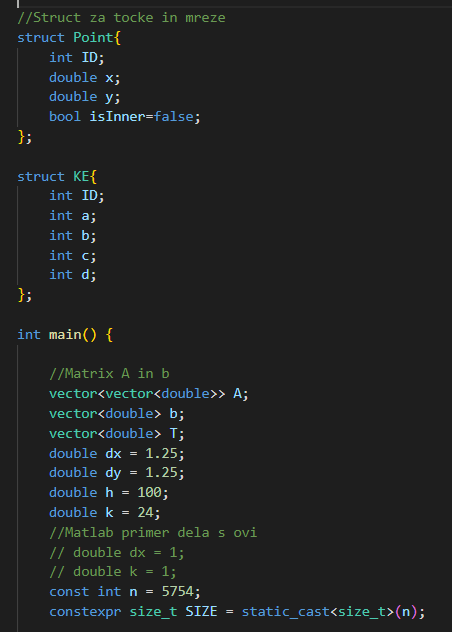
\includegraphics[width=0.5\linewidth]{declare.png}
        \renewcommand*\figurename{Slika}
        \caption{Struct za točke in mreže}
        \label{Slika:1}
    \end{figure}

\FloatBarrier
\subsection{Branje podatkov}
    Podatki za naš problem so podani v datoteki primer2mreza.txt, katero beremo. Podatke o točkah vstavimo pa v \textbf{vector$<$Point$>$ points}. Iz podatkov mreže pa generiramo adjacency matriko, katera nam pomaga pri določanju okolice za vsako točko.

    \begin{figure}[ht]
        \centering
        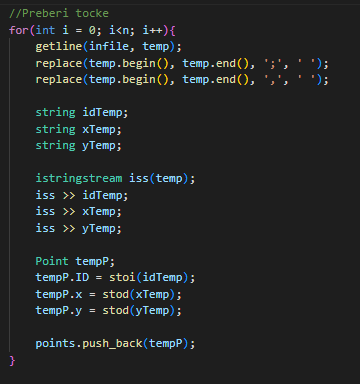
\includegraphics[width=0.2\linewidth]{preberiTocke.png}
        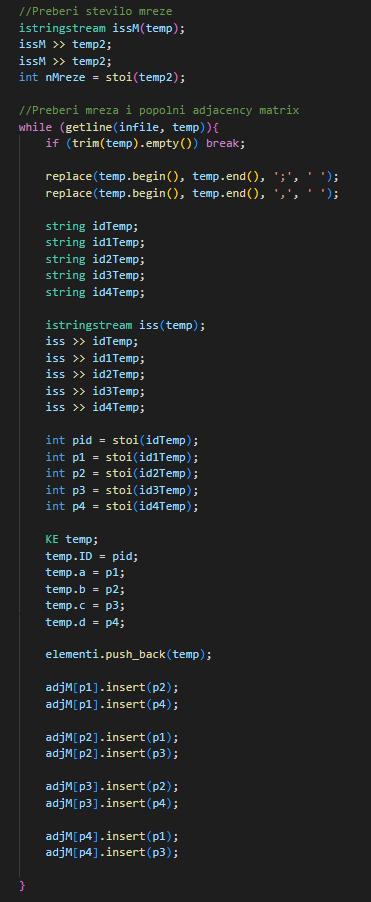
\includegraphics[width=0.2\linewidth]{preberiMrezeinadjM.png}
        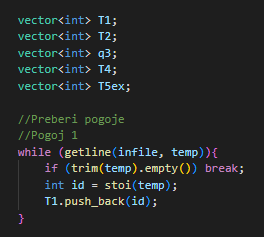
\includegraphics[width=0.5\linewidth]{preberemePogoji.png}
        \renewcommand*\figurename{Slika}
        \caption{Branje podatkov iz datoteke primer2mreza.txt}
        \label{Slika:2}
    \end{figure}
\FloatBarrier
\subsection{Preverjanje notranjih točk}
    Preveriti je potrebno tudi, pozicijo točk, ali je točka notranja, kar nam je pomembno v nadaljevanju pri generaciji matrik A in b. To pa naredimo s kodo na \textit{Slika 3}.
    \begin{figure}[ht]
        \centering
        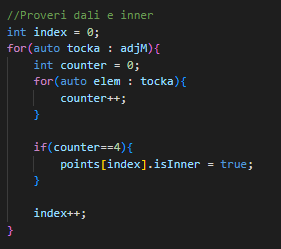
\includegraphics[width=0.3\linewidth]{isInner.png}
        \renewcommand*\figurename{Slika}
        \caption{Preverjanje notranjih točk}
        \label{Slika:3}
    \end{figure}
\FloatBarrier
\subsection{Inicializiranje matrik A, b, T}
    Za optimizacijo in skrajševanje časa izvedbe programa, najprej inicializiramo A, b, T. T pa polnimo s 100, kar pa je naša začetna predpostavka.
        \begin{figure}[ht]
        \centering
        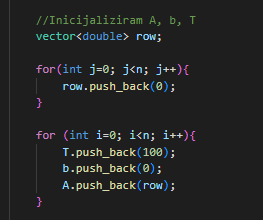
\includegraphics[width=0.5\linewidth]{inicijalizacijaAbT.png}
        \renewcommand*\figurename{Slika}
        \caption{Inicializacija matrik A, b, T}
        \label{Slika:4}
    \end{figure}
\FloatBarrier
\subsection{Ispolnjevanje matrik A, b}
    Za reševanje problema potrebno je matrike A in b isponiti z robnimi pogoji in enačbami za notranje točke.
    \FloatBarrier
    \subsubsection{Pogoj 1}
    Pogoj 1 - podadene točke imajo temperaturo 400$^oC$
    \begin{figure}[ht]
        \centering
        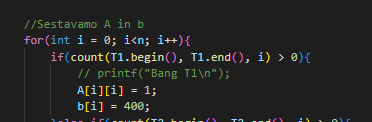
\includegraphics[width=0.5\linewidth]{pogoj1.png}
        \renewcommand*\figurename{Slika}
        \caption{Pogoj 1}
        \label{Slika:5}
    \end{figure}
    \FloatBarrier
    \subsubsection{Pogoj 2}
        Pogoj 2 - podadene točke imajo temperaturo 100$^oC$
            \begin{figure}[ht]
                \centering
                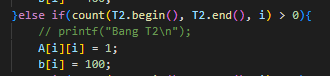
\includegraphics[width=0.5\linewidth]{pogoj2.png}
                \renewcommand*\figurename{Slika}
                \caption{Pogoj 2}
                \label{Slika:6}
            \end{figure}
    \FloatBarrier
    \subsubsection{Pogoj 3}
        Pogoj 3 nam pove da v določenih točkah na robu imamo podan toplotni tok. Za to smo uporabili naslednjo enačbo. 
        $$(2T_{m-1,n}+T_{m,n-1}+T_{m,n+1})+2\frac{q\Delta x}{k}-4T_{m,n}=0$$
        Točko \(T_{m-1,n}\) smo spomočjo isIner ugotovili, če je notranja točka ter smo jo množili z 2, sosednje točke pa smo množili z 1. Kjer je q=0, četrti član je enak 0.
            \begin{figure}[ht]
                \centering
                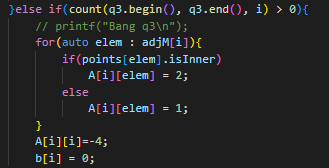
\includegraphics[width=0.5\linewidth]{pogoj3.png}
                \renewcommand*\figurename{Slika}
                \caption{Pogoj 3}
                \label{Slika:7}
            \end{figure}
    \FloatBarrier
    \subsubsection{Pogoj 4}
         Pogoj 4 - podadene točke imajo temperaturo 600$^oC$
        \begin{figure}[ht]
            \centering
            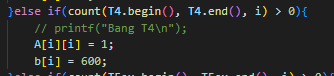
\includegraphics[width=0.7\linewidth]{pogoj4.png}
            \renewcommand*\figurename{Slika}
            \caption{Pogoj 4}
            \label{Slika:8}
        \end{figure}
\newpage
        \FloatBarrier
 \subsubsection{Pogoj 5}
        Pogoj 5 - Prestop toplote.\newline
        Najprej preverimo ali je točka na robu ali pa je notranja. To preverimo s isInner, kar nam poda True za notranje točke. Za notranje točke pa uporabimo sledečo enačbo
        $$2(T_{m-1,n}+T_{m,n+1})+(T_{m+1,n}+T_{m+,n-1})+2\frac{h \Delta x}{k}T_{ext}-2(3+\frac{h\Delta x}{k})T_{m,n}=0$$
        Za točke na robu moramo uporabiti drugo enačbo, in sicer:
        $$2(T_{m-1,n}+T_{m,n+1}+T_{m,n-1})+2\frac{h\Delta x}{k}T_{ext}-2(\frac{h\Delta x}{k}+2)T_{m,n}=0$$
            \begin{figure}[ht]
                \centering
                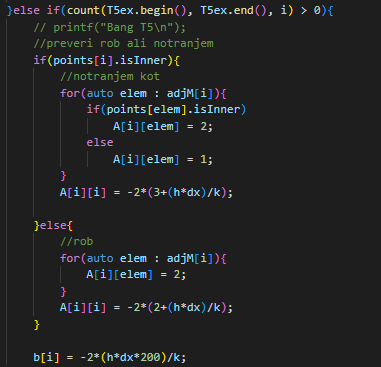
\includegraphics[width=0.5\linewidth]{pogoj5.png}
                \renewcommand*\figurename{Slika}
                \caption{Pogoj 5}
                \label{Slika:9}
            \end{figure}
        \FloatBarrier
\subsubsection{Notranje točke}
     Vse točke, ki nimajo podanega nekega pogoja so notranje. Za njih pa velja enačba 
        $$T_{m-1,n}+T_{m+1,n}+T_{m,n-1}+T_{m,n+1}-4T_{m,n}=0$$
            \begin{figure}[ht]
                \centering
                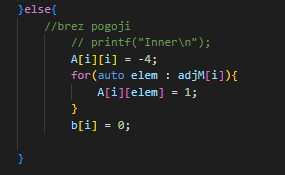
\includegraphics[width=0.5\linewidth]{ostaliPogoji.png}
                \renewcommand*\figurename{Slika}
                \caption{Enačba za notranje točke}
                \label{Slika:10}
            \end{figure}
    \FloatBarrier
\subsection{Gauss-Seidl metoda}
    Pri pojektu smo uporabili Gauss-Seidelovo metodo podobno, kot pri domači nalogi 4, kjer smo paralelizirali kalkulacije po vrsti. V paralelizaciji smo pa uporabili maksimalno število threadov.
            \begin{figure}[ht]
                \centering
                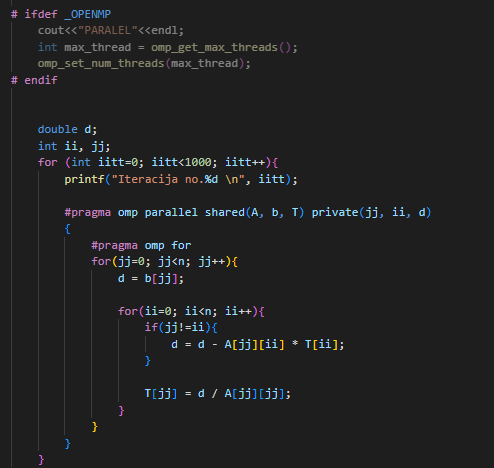
\includegraphics[width=0.5\linewidth]{gauss_paralelizacija.png}
                \renewcommand*\figurename{Slika}
                \caption{Gauss-Seidl}
                \label{Slika:11}
            \end{figure}
\FloatBarrier
\subsection{Shranjevanje rešitev v VTK format}
    Rešitev smo shranili v .vtk datoteko, da bi jo lahko uvozili v program ParaView ter vizualizirali našo rešitev. Format rezultata je zasnovan na rezultat\_vtk.vtk iz primera.
        \begin{figure}[ht]
            \centering
            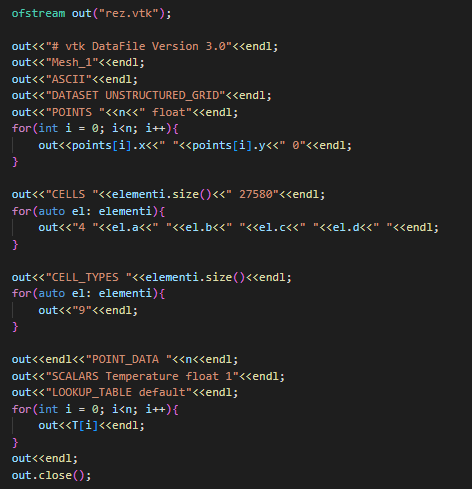
\includegraphics[width=0.5\linewidth]{generateVtk.png}
            \renewcommand*\figurename{Slika}
            \caption{Generacija .vtk datoteke}
            \label{Slika:12}
        \end{figure}
\FloatBarrier
\section{ParaView}
Generiran vtk file smo vizualizirali v programu ParaView. 
\newline Nalogo smo tudi za primerjavo rešili v MATLAB programskemu jeziku. Opomba: primer rešen v MATLAB-u, v kod je bilo deklarirano, da je dx=1 in k=1, kar v našem primeru ni točno, kajti v našem primeru je dx=1.25 in k=24, zato se rešitvi razlikujeta.
\newline Nalogo smo tudi za primerjavo rešili v MatLab programskemu jeziku.(desno)
    \begin{figure}[ht]
        \centering
        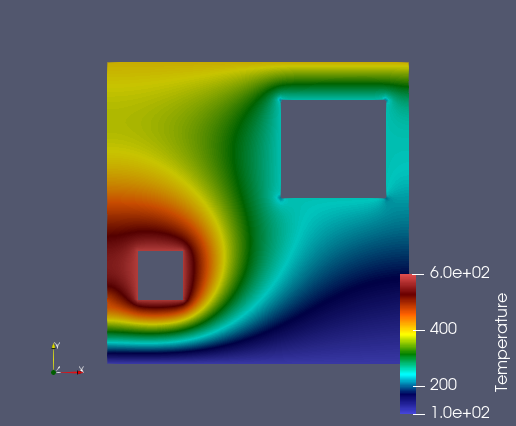
\includegraphics[width=0.35\linewidth]{paraview.png}
        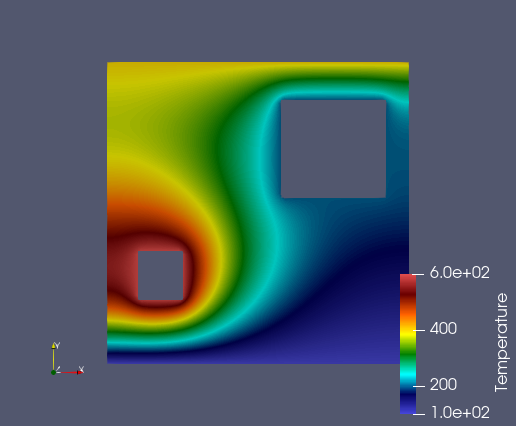
\includegraphics[width=0.35\linewidth]{rezMatlab.png}
        \renewcommand*\figurename{Slika}
        \caption{Primerjava rešitev naloge C++ in MATLAB v ParaView}
        \label{Slika:13}
    \end{figure}

\newpage
\FloatBarrier
\section{Analiza}

\subsection{Primerjava hitrosti izvajanja prograva v C++ in MATLAB}

Za Gauss-Seidel metodo smo naredili 1000 iteracij ter istočasno preverili koliko časa potrebujemo za izvedbo. To smo naredili s 1, 2, 3, 4, 5, 6, 7 threadov v C++ in serijski oziroma s 1 thread v MATLAB (kjer Parallel Computing Toolbox ni delal in nismo mogli uporabiti parafor)
\newline
Rezultat ki ga dobimo pri serijskem reševanju v C++ je 677s, v MATLAB-u pa je 285s. Iz rezultata pa je razvidno da je MATLAB hitrejši, ker bolj efikasno uporablja memorijo ter ima vgrajeno optimizacijo. Z boljšo optimizacijo našega programa bi lahko v C++ dobili hitreše rezultat, ker je nižji programski jezik in "lightweight".
            \begin{figure}[ht]
                \centering
                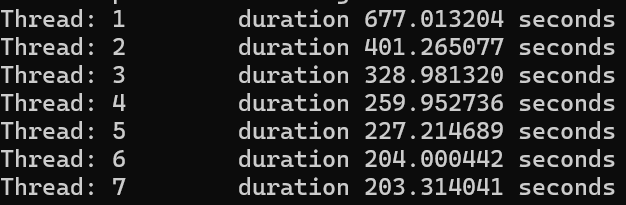
\includegraphics[width=0.4\linewidth]{paralel.png}
                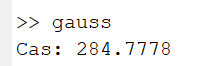
\includegraphics[width=0.4\linewidth]{casMATLAB.png}
                \renewcommand*\figurename{Slika}
                \caption{Primerjava hitrosti programov}
                \label{Slika:14}
            \end{figure}
\FloatBarrier
\subsubsection{Strong scaling}
Rezultete časov komputacije različnega števila threadov(niti) lahko primerjamo v grafu strong scaling. Vidimo, da odstopamo od idealne (oranžne) črte, kar je normalno. Naš cilj je, da našo izmerjeno linijo (modro) čim bolj približamo idealni. Ideja idealne linije je, da lahko z uporabo N threadov omogočimo N-krat hitrejše izvajanje našega programa. V resnici to ni mogoče.
            \begin{figure}[ht]
                \centering
                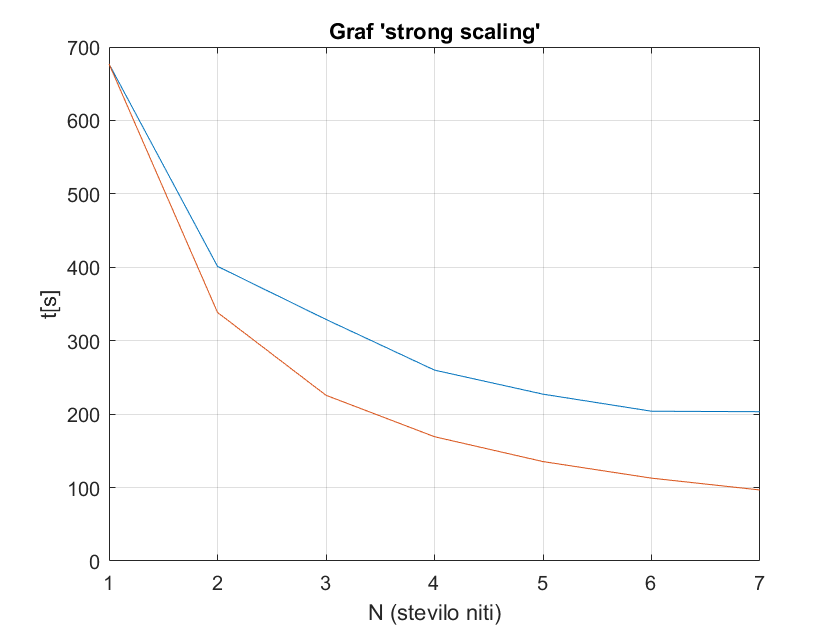
\includegraphics[width=\linewidth]{strongscaling.png}
                \renewcommand*\figurename{Slika}
                \caption{Strong scaling graf}
                \label{Slika:15}
            \end{figure}

\end{document}